% !TeX program = xelatex
% This paper follows the LLNCS macro package for Springer Computer Science
% proceedings; based on samplepaper.tex, Version 2.21 of 2022/01/12.
%
% Ban tieng Viet duoc dong bo noi dung voi ban nop tieng Anh hien hanh.
%
% Bo cuc: Gioi thieu, Cong trinh lien quan, Phuong phap, Thuc nghiem
% (thiet lap, bang chinh, doi sanh, luoi, ablation, do nhay, han che), Ket luan.
%
\documentclass[runningheads]{llncs}
%
% Unicode fonts supplied with TeX Live / Overleaf. Compile with XeLaTeX.
\usepackage{iftex}
\ifXeTeX\else
  \PackageError{soict2026}{Select XeLaTeX as the compiler}{In Overleaf settings,
  select XeLaTeX, then Recompile from scratch.}
\fi
\usepackage[no-math]{fontspec}
\setmainfont{Latin Modern Roman}
\setsansfont{Latin Modern Sans}
\setmonofont{Latin Modern Mono}
%
\usepackage{graphicx}
\usepackage{amsmath}
\usepackage{amssymb}
\usepackage{url}
\usepackage{booktabs}
\usepackage{pgfplots}
\pgfplotsset{compat=1.18}
\definecolor{plotblue}{RGB}{43,99,151}
\definecolor{plotteal}{RGB}{23,126,110}
\definecolor{plotpurple}{RGB}{111,79,156}
\definecolor{plotorange}{RGB}{194,105,32}
% The pipeline figure is drawn in TikZ, i.e. vector graphics, as the sample
% recommends for diagrams and schematics.
\usepackage{tikz}
\usetikzlibrary{arrows.meta, positioning, calc, fit, backgrounds}
% The figure uses functional colour groups and native vector geometry.
% The photograph lives in figure_assets/ in the repository; Overleaf expects it
% beside the source, so the path is searched in both places.
\graphicspath{{./}{figure_assets/}}
% Keep the source compilable when it is pasted into Overleaf without the
% optional photograph.  The complete upload package still includes the image.
\newcommand{\mallardimage}[1]{%
  \IfFileExists{mallard.jpg}{%
    \includegraphics[width=#1]{mallard.jpg}%
  }{%
    \IfFileExists{figure_assets/mallard.jpg}{%
      \includegraphics[width=#1]{figure_assets/mallard.jpg}%
    }{%
      \fcolorbox{plotblue}{blue!5}{%
        \resizebox{#1}{!}{\strut\textsf{Vịt trời}}}%
    }%
  }%
}
% Hien thi tieu de tom tat can giua theo kieu cua ban nop.
\renewenvironment{abstract}{%
  \par\addvspace{.35cm}%
  \begin{center}\large\bfseries\abstractname\end{center}%
  \vspace{-.5em}%
  \list{}{\small
    \setlength{\leftmargin}{1cm}%
    \setlength{\rightmargin}{1cm}%
    \setlength{\labelwidth}{0pt}%
    \setlength{\listparindent}{0pt}%
    \setlength{\itemindent}{0pt}%
    \setlength{\topsep}{0pt}%
    \setlength{\partopsep}{0pt}%
    \setlength{\parsep}{0pt}%
    \setlength{\itemsep}{0pt}}%
  \item\relax
}{\endlist}
%
\begin{document}
%
\renewcommand{\andname}{và}
\renewcommand{\abstractname}{Tóm tắt}
\renewcommand{\keywordname}{{\bf Từ khóa:}}
\renewcommand{\figurename}{Hình}
\renewcommand{\tablename}{Bảng}
\renewcommand{\refname}{Tài liệu tham khảo}
\renewcommand{\proofname}{Chứng minh}
\renewcommand{\ackname}{Lời cảm ơn.}
%
\title{Hợp nhất hai tầng cho định tuyến và phân lớp trong
học liên tục hiệu quả tham số}
%
\titlerunning{Hợp nhất hai tầng cho học liên tục dựa trên PET}
%
% ORCID iDs not yet available; \orcidID{} omitted for now. Fill in before
% the final submission.
\author{Nguyễn Thiên Trường \and Tống Quang Thái}
%
\authorrunning{N. T. Trường và T. Q. Thái}
%
\institute{Trường Đại học Công nghệ, Đại học Quốc gia Hà Nội,\\
Hà Nội, Việt Nam\\
\email{24022480@vnu.edu.vn, 24022450@vnu.edu.vn}}
%
\maketitle
% SOICT 2026 submission: keep author identities, suppress page numbers.
\pagestyle{empty}
\thispagestyle{empty}
%
\begin{abstract}
Học liên tục hiệu quả tham số có thể bảo toàn mạng xương sống tiền huấn luyện
bằng cách gán các bộ điều hợp gọn nhẹ cho những tác vụ lần lượt xuất hiện. Tuy
nhiên, trong thiết lập không biết tác vụ, suy luận gắn hai quyết định khác nhau:
lựa chọn bộ điều hợp và nhận dạng một lớp trong toàn bộ các lớp đã thấy. Hai
quyết định này không tương đương, nên sửa định tuyến có thể không đổi kết quả
phân lớp hoặc làm hỏng một dự đoán vốn đã đúng. Chúng tôi xử lý sự lệch này bằng
một khung hợp nhất hai tầng, bổ sung vào pipeline dựa trên bộ điều hợp một đầu
ridge chiếu ngẫu nhiên (RP) mang bằng chứng bổ trợ. Đầu RP hoạt động trong một
không gian đặc trưng cố định và được cập nhật từ các thống kê bậc hai cộng dồn,
không lưu mẫu cũ và không thêm cập nhật gradient cho các bộ điều hợp hiện có.
Điểm RP trước hết sửa đề xuất tác vụ trước bước đối sánh lại, sau đó hỗ trợ hợp
nhất có xét độ tin cậy với logit lớp cuối. Đánh giá trên nhiều bộ dữ liệu, seed
và thiết lập tiền huấn luyện xem xét riêng định tuyến, phân lớp và khả năng ghi
nhớ, qua đó cho thấy hai nguồn bằng chứng bổ sung cho nhau nhưng tác động vẫn
phụ thuộc cấu hình.

\keywords{Học liên tục \and Tinh chỉnh hiệu quả tham số \and Định tuyến tham số
\and Chiếu ngẫu nhiên \and Hợp nhất tín hiệu.}
\end{abstract}
%
%
%
\section{Giới thiệu}

Học liên tục yêu cầu mô hình tiếp nhận một chuỗi tác vụ mà không đánh mất kiến
thức đã học trước đó. Tinh chỉnh hiệu quả tham số thích nghi một mạng xương sống
tiền huấn luyện đóng băng bằng một lượng nhỏ tham số. Một họ phương pháp quan
trọng duy trì prompt hoặc bộ điều hợp riêng cho từng tác vụ và lựa chọn chúng
khi suy luận~\cite{ref_dualprompt,ref_hide}. Các phương pháp này có thể không
lưu mẫu cũ, nhưng bảo toàn tham số không đồng nghĩa với bảo toàn độ chính xác.

Trong họ này, định danh tác vụ không được biết khi suy luận và việc chọn tham
số tự nó là một bài toán dự đoán. Bộ điều hợp sai có thể tạo ra đặc trưng không
phù hợp. Kho lớn hơn, tổ hợp có trọng số attention và đối sánh lại tường minh
là các hướng xử lý khác nhau~\cite{ref_l2p,ref_coda,ref_hrmpet}. Tuy nhiên,
chọn bộ điều hợp phù hợp hơn và dự đoán đúng lớp là hai mục tiêu khác nhau:
đầu phân lớp dùng chung có thể khôi phục sau lỗi định tuyến, còn thay đổi định
tuyến cũng có thể phá một dự đoán vốn đã đúng.

Chúng tôi bổ sung một bộ dự đoán hỗ trợ gồm đặc trưng từ bộ điều hợp tác vụ đầu,
phép chiếu ngẫu nhiên đóng băng và bộ phân lớp ridge được khớp từ thống kê cộng
dồn theo RanPAC~\cite{ref_ranpac}. Việc khớp chỉ dùng dữ liệu tác vụ hiện tại,
không thay đổi huấn luyện LoRA/TII và không lưu mẫu. Điểm số của nó sửa đề xuất
tác vụ trước đối sánh lại rồi được trộn với logit lớp cuối, với trọng số lớn hơn
khi biên giữa hai lớp đứng đầu của bộ phân lớp chính nhỏ đi.

\subsubsection{Đóng góp.}
Chúng tôi đóng góp (i) một bộ dự đoán RP dùng chung cho hợp nhất đề xuất tác vụ
và hợp nhất lớp có cổng biên, (ii) các đối chứng cùng đặc trưng và ablation có
điều kiện trên bốn seed, và (iii) khảo sát bốn bộ dữ liệu, năm thiết lập tiền
huấn luyện cùng phân tích độ nhạy trọng số. Điểm mới nằm ở cách tích hợp tại hai
điểm quyết định và đánh giá nó, không phải bản thân hồi quy ridge. Chúng tôi
phân biệt mức tăng phân lớp với khả năng ghi nhớ, và khả năng bổ sung oracle
với các sửa chữa thực sự đạt được.

\section{Công trình liên quan}
\label{sec:related}

\subsubsection{Kho tham số và yêu cầu lựa chọn.}
L2P~\cite{ref_l2p} và DualPrompt~\cite{ref_dualprompt} dùng truy vấn từ mạng
xương sống đóng băng để chọn tham số nhẹ trong một kho. CODA-Prompt
~\cite{ref_coda} kết hợp prompt bằng trọng số attention. HiDe-Prompt
~\cite{ref_hide} tách dự đoán trong tác vụ, suy luận định danh tác vụ và dự
đoán thích nghi theo tác vụ, đồng thời chỉ ra suy luận định danh là nút thắt.
HRM-PET~\cite{ref_hrmpet} dùng bộ điều hợp LoRA~\cite{ref_lora} và đối sánh lại
để xem xét lại lựa chọn ban đầu. MoTE~\cite{ref_mote} kết hợp các chuyên gia
theo tác vụ; DLEPEM~\cite{ref_dlepem} kết hợp prototype chung và prototype đã
thích nghi để đối sánh.

\subsubsection{Nghiệm dạng đóng trong học liên tục.}
Bộ phân lớp dạng đóng bảo toàn đóng góp cũ thông qua thống kê cộng dồn của đặc
trưng cố định. APER~\cite{ref_adam} thích nghi mạng xương sống ở tác vụ đầu,
sau đó dùng đặc trưng đóng băng và prototype lớp. ACIL~\cite{ref_acil} dùng
bình phương tối thiểu đệ quy, thay bộ đệm mẫu bằng thống kê tương quan và khôi
phục nghiệm chung tương ứng. DS-AL~\cite{ref_dsal} thêm một luồng giải tích thứ
hai. RanPAC~\cite{ref_ranpac} áp dụng phép chiếu ngẫu nhiên cố định lên đặc
trưng đóng băng, cộng dồn thống kê bậc hai và giải hệ ridge.

Chúng tôi kế thừa phép chiếu, phép cộng dồn Gram và lời giải ridge của RanPAC,
nhưng giữ quy trình định tuyến bộ điều hợp và tham khảo đầu này tại hai điểm
quyết định thay vì dùng nó làm bộ dự đoán duy nhất.

\subsubsection{Hiệu chỉnh bộ phân lớp sau huấn luyện.}
Học tăng dần theo lớp thường thiên lệch dự đoán về các lớp gần đây
~\cite{ref_survey}. iCaRL~\cite{ref_icarl} dùng trung bình exemplar gần nhất;
BiC~\cite{ref_bic} học hiệu chỉnh logit affine trên dữ liệu giữ lại; Weight
Aligning~\cite{ref_wa} khớp chuẩn trọng số của lớp mới và cũ; LUCIR
~\cite{ref_lucir} chuẩn hóa đặc trưng và trọng số. Phép hợp nhất của chúng tôi
giữ cố định các bộ điều hợp, đầu phụ và đầu dùng chung. Nó không giữ exemplar
nhưng cần dữ liệu tác vụ hiện tại để khớp đầu RP.

\subsubsection{Thách thức còn lại.}
Sự không nhất quán prompt/bộ phân lớp giữa huấn luyện và kiểm thử có thể làm
giảm chất lượng dự đoán~\cite{ref_cprompt}; đối sánh lại xử lý lựa chọn tham số
nhưng không cung cấp một bộ dự đoán lớp độc lập. Chúng tôi tiếp nhận giao diện
đối sánh lại của HRM-PET~\cite{ref_hrmpet}, giữ nguyên việc huấn luyện bộ điều
hợp và bộ phân lớp, rồi thử bằng chứng RP bổ sung trước và sau đối sánh lại.
Điều này khác với thay thế việc chọn bộ điều hợp bằng một bộ phân lớp giải tích.

\section{Phương pháp}
\label{sec:method}

\subsection{Phát biểu bài toán}

Học tăng dần theo lớp (CIL) nhằm học $T$ tác vụ đồng thời giảm quên. Tác vụ
$t$ cung cấp các ảnh có nhãn
$\mathcal D_t=\{(x_i^t,y_i^t)\}_{i=1}^{n_t}$ từ tập lớp $\mathcal C_t$,
với $\mathcal C_t\cap\mathcal C_{t'}=\emptyset$ khi $t\ne t'$. Chỉ dữ liệu
tác vụ hiện tại được dùng để huấn luyện; ảnh cũ không bao giờ được giữ lại.
Khi suy luận, định danh tác vụ không biết trước và dự đoán trải trên mọi lớp
đã thấy.

Thiết lập PET theo tác vụ của chúng tôi~\cite{ref_hide,ref_hrmpet} đóng băng
tham số mạng xương sống $\theta_{\mathrm{ptm}}$ và duy trì các bộ điều hợp LoRA
$\mathcal P=\{p_1,\dots,p_T\}$, mỗi tác vụ một bộ, cùng đầu phân lớp dùng chung
$g_{\theta_g}$. Dự đoán chính cần chọn bộ điều hợp; nhánh RP cố định độc lập với
tác vụ được suy ra.

Chúng tôi phân biệt bốn vector điểm lớp: điểm TII trần $u$, logit đầu dùng chung
sau lượt thích nghi ban đầu $r$, logit sau đối sánh lại cuối cùng $\ell$, và
điểm RP $s$. Ánh xạ từ lớp sang tác vụ là $\mathcal T(\cdot)$. Đầu phụ
$g_\omega$ ánh xạ đặc trưng trần thành $u$, cho
$t_0=\mathcal T(\arg\max_c u_c)$. Lượt thích nghi ban đầu cho
$r=g(\phi(x;p_{t_0}))$. DRM chỉ đánh giá bộ điều hợp được đề xuất khi
$\hat t_{\rm DRM}\ne t_0$. CRM dùng độ tin cậy entropy tổng quát của $r$, thử
tác vụ chứa lớp xếp thứ hai, rồi giữ logit theo log-sum-exp; nó không bị giới
hạn bởi sự đồng thuận giữa các đề xuất tác vụ và không chạy ở tác vụ 1. Mọi
lượt thích nghi dùng chung $g$; $\ell$ là logit lớp được giữ lại. Ký hiệu
$z(\cdot)$ là chuẩn hóa theo từng mẫu, với độ lệch chuẩn tổng thể có ngưỡng dưới
$10^{-6}$.

\begin{figure}[!t]
\centering
% Original scientific artwork; photos are documented in FIGURE_SOURCES.txt.
\definecolor{ib}{RGB}{43,99,151}%
\definecolor{it}{RGB}{23,126,110}%
\definecolor{ip}{RGB}{111,79,156}%
\definecolor{io}{RGB}{194,105,32}%
\definecolor{ir}{RGB}{172,63,99}%
\newcommand{\snowmark}{%
  \tikz[baseline=-.55ex,x=.11em,y=.11em,line cap=round]{%
    \foreach \a in {0,60,...,300}{%
      \draw[ib,line width=.48pt] (0,0)--(\a:4.3);
      \draw[ib,line width=.32pt] (\a:2.8)--({\a+24}:3.8);
      \draw[ib,line width=.32pt] (\a:2.8)--({\a-24}:3.8);
    }}}
\newcommand{\firemark}{%
  \tikz[baseline=-.55ex,x=.09em,y=.09em]{%
    \path[fill=io]
      (0,-4.8) .. controls (-4.0,-2.2) and (-2.2,1.2) .. (-1.1,4.7)
      .. controls (-.2,2.8) and (1.8,2.3) .. (2.4,5.1)
      .. controls (5.0,1.1) and (4.0,-2.6) .. (0,-4.8) -- cycle;
    \path[fill=yellow!75!orange]
      (.15,-4.0) .. controls (-1.6,-2.2) and (-.5,-.2) .. (.7,1.8)
      .. controls (2.5,-.6) and (2.6,-2.5) .. (.15,-4.0) -- cycle;}}
\newcommand{\analyticmark}{\textcolor{ip}{\(\boldsymbol{\Sigma}\)}}
\begin{tikzpicture}[x=1cm,y=1cm,
  font=\fontsize{8}{9}\selectfont,
  arr/.style={-{Stealth[length=1.5mm]},line width=.6pt,draw=ib},
  tinylabel/.style={font=\fontsize{7}{8}\selectfont,align=center},
  heading/.style={anchor=west,font=\fontsize{8}{9}\selectfont\bfseries},
  dot/.style={circle,inner sep=0pt,minimum size=1.4mm},
  pics/vit/.style args={#1/#2}{
    code={
      \foreach \k in {3,2,1,0}{
        \draw[draw=#1!80,fill=#1!10,line width=.45pt]
          ({-.43+.09*\k},{-.36+.07*\k}) rectangle
          ({.24+.09*\k},{.36+.07*\k});
      }
      \foreach \y in {-.22,.23}{
        \draw[#1!65,line width=.3pt] (-.34,\y) -- (.14,\y);
      }
      \node[tinylabel] at (-.05,-.03) {ViT};
      \node[tinylabel,text=#1] at (.02,-.64) {#2};
    }},
  pics/matrix/.style args={#1/#2}{
    code={
      \foreach \i in {0,...,4}\foreach \j in {0,...,4}{
        \pgfmathtruncatemacro{\shade}{15+mod(13*\i+29*\j,65)}
        \fill[#1!\shade] ({-.35+.14*\i},{-.35+.14*\j})
             rectangle ++(.13,.13);
      }
      \draw[#1,line width=.4pt] (-.36,-.36) rectangle (.35,.35);
      \node[tinylabel,text=#1] at (0,-.58) {#2};
    }},
  pics/net/.style={
    code={
      \foreach \a in {-.3,0,.3}\foreach \b in {-.45,-.225,0,.225,.45}{
        \draw[it!30,line width=.22pt] (-.42,\a) -- (.42,\b);
      }
      \foreach \a in {-.3,0,.3}
        \node[dot,draw=it,fill=it!20] at (-.42,\a) {};
      \foreach \b in {-.45,-.225,0,.225,.45}
        \node[dot,draw=it,fill=it!65] at (.42,\b) {};
    }}
]
% Three aligned lanes; fusion details stay inside their own coloured panels.
\path[use as bounding box] (0,-.03) rectangle (12.1,9.52);
\node[heading,text=io] at (0,9.30) {(a) Học PET trên tác vụ $t$};
\node[tinylabel,anchor=east,text=black!65] at (12.1,9.30)
  {\snowmark\ Cố định \quad \firemark\ Huấn luyện \quad
   \analyticmark\ Giải tích};
\node[inner sep=0pt] at (.48,8.63) {\mallardimage{.72cm}};
\node[tinylabel] at (.48,8.13) {$\mathcal D_t$};
\draw[arr,draw=io] (.96,8.63) -- (1.30,8.63);
\node[tinylabel,draw=ib,fill=ib!7,minimum width=2.35cm,minimum height=.55cm]
  at (2.50,8.63) {\snowmark\ ViT tiền huấn luyện};
\node[tinylabel,text=black!60] at (4.05,8.63) {$+$};
\node[tinylabel,draw=io,fill=io!9,minimum height=.55cm,inner xsep=6pt]
  at (5.65,8.63) {\firemark\ $p_t$, các đầu $g$, $g_\omega$};
\node[tinylabel,draw=ib,fill=ib!7,minimum width=2.50cm,minimum height=.55cm]
  at (9.55,8.63) {\snowmark\ Các $p_{<t}$ cũ};
\draw[black!20,line width=.35pt] (0,7.88) -- (12.1,7.88);
\node[heading,text=ib] at (0,7.49) {(b) \snowmark\ Suy luận};
% Main inference lane.
\node[inner sep=0pt] (input) at (.52,6.15)
  {\mallardimage{.94cm}};
\node[tinylabel] at (.52,6.86) {Đầu vào $x$};
\draw[arr] (1.04,6.15) -- (1.48,6.15);
\pic at (1.95,6.11) {vit={ib/{\fontsize{6.6}{7.2}\selectfont ViT trần\hspace{2pt}+\hspace{2pt}$g_\omega$}}};
\draw[arr] (2.50,6.15) -- node[tinylabel,above] {$u\mapsto t_0$} (3.48,6.15);
\pic at (3.95,6.11) {vit={ib/{\fontsize{6.6}{7.2}\selectfont $p_{t_0}$\hspace{2pt}+\hspace{2pt}đầu $g$}}};
\node[tinylabel,draw=ib,fill=ib!12,inner xsep=2pt,inner ysep=2pt]
  (adapter) at (3.95,7.00)
  {\snowmark\ LoRA $p_{t_0}$};
\draw[arr] (adapter.south) -- (3.95,6.63);
\draw[arr] (4.50,6.15) -- node[tinylabel,above] {$r$} (4.92,6.15);
% Stage 1: both sources receive the same task-level reduction and scaling.
\draw[io!70,fill=io!5,rounded corners=3pt,line width=.7pt]
  (4.92,5.08) rectangle (6.62,6.84);
\node[font=\fontsize{6.8}{7.4}\selectfont,text=io] at (5.77,6.58)
  {\textbf{1 Định tuyến}};
\draw[io!25] (5.04,6.36) -- (6.50,6.36);
\node[font=\fontsize{6.8}{7.4}\selectfont,align=center] at (5.77,5.77)
  {Max tác vụ\\Trộn $w$\\Argmax};
\draw[arr,draw=io] (6.62,6.15) -- node[tinylabel,above] {$\hat t_{\rm DRM}$} (7.56,6.15);
\pic at (8.03,6.11) {vit={ib/{\fontsize{6.6}{7.2}\selectfont DRM\hspace{1.5pt}/\hspace{1.5pt}CRM\hspace{2pt}+\hspace{2pt}$g$}}};
\draw[arr] (8.58,6.15) -- node[tinylabel,above] {$\ell$} (9.18,6.15);
% Stage 2: the gate is internal, avoiding an extra crossing control wire.
\draw[ir!70,fill=ir!5,rounded corners=3pt,line width=.7pt]
  (9.22,5.10) rectangle (10.94,6.82);
\node[tinylabel,text=ir] at (10.08,6.57) {\textbf{2 Phân lớp}};
\draw[ir!25] (9.35,6.36) -- (10.81,6.36);
\node[tinylabel] at (10.08,5.78)
  {Cổng$(\ell)$ $\rightarrow z$\\Trộn $\beta_i$\\Đổi thang};
\draw[arr,draw=ir] (10.94,6.15) -- (11.35,6.15);
\node[inner sep=0pt] at (11.73,6.15)
  {\mallardimage{.66cm}};
\node[tinylabel,text=ir] at (11.73,5.50) {$\hat y$:\\Mallard};
% Second lane: RP features, expansion and class-score profile.
\node[heading,text=it] at (.20,4.82)
  {\snowmark\ Nhánh RP: $p_1$, thêm một lượt};
\draw[arr,draw=it] (input.south) -- (.52,5.18) -- (.07,5.18) --
  (.07,3.89) -- (1.40,3.89);
\draw[draw=ib!70,fill=ib!3,rounded corners=2pt,line width=.5pt]
  (1.40,3.34) rectangle (2.74,4.66);
\pic at (2.03,3.82) {vit={it/$p_1$}};
\node[font=\fontsize{6.8}{7}\selectfont,text=ib,anchor=north west,inner sep=0pt]
  at (1.47,4.58) {\snowmark};
\draw[arr,draw=it] (2.74,3.89) -- (2.99,3.89);
\foreach \k/\tone in {0/20,1/65,2/40,3/85}{
  \fill[it!\tone] (3.10,{3.52+.18*\k}) rectangle ++(.21,.17);
}
\node[tinylabel,text=it] at (3.21,3.20) {$f$\\768};
\draw[arr,draw=it] (3.43,3.89) -- (3.76,3.89);
\draw[draw=ib!70,fill=ib!3,rounded corners=2pt,line width=.5pt]
  (3.76,3.40) rectangle (5.08,4.66);
\pic at (4.42,3.95) {net};
\node[font=\fontsize{6.5}{7}\selectfont,align=center,text=it]
  at (4.42,3.14) {$W^\top$\\ReLU};
\node[font=\fontsize{6.4}{6.8}\selectfont,text=ib,anchor=north west,inner sep=0pt]
  at (3.83,4.58) {\snowmark};
\draw[arr,draw=it] (5.08,3.89) -- (5.37,3.89);
\foreach \k in {0,...,7}{
  \pgfmathtruncatemacro{\tone}{12+mod(31*\k,75)}
  \fill[it!\tone] (5.48,{3.46+.115*\k}) rectangle ++(.23,.105);
}
\node[tinylabel,text=it] at (5.60,3.20) {$h$\\$10^4$};
\draw[arr,draw=ip] (5.83,3.89) -- (6.36,3.89);
\pic at (6.85,3.89) {matrix={ip/$W_{\rm out}$}};
\draw[arr,draw=ip] (7.32,3.89) -- (7.60,3.89);
\foreach \pos/\height in {7.69/.57,8.01/.23,8.33/.13,8.65/.10}{
  \fill[ip!75] (\pos,3.63) rectangle ++(.15,\height);
}
\draw[ip!70,line width=.3pt] (7.62,3.61) -- (8.88,3.61);
\node[tinylabel,text=ip] at (8.255,3.12) {Điểm $s$};
\foreach \pos/\lab in {7.765/1,8.085/2,8.405/3,8.725/4}{
  \node[font=\fontsize{6}{7}\selectfont,text=ip,inner sep=0pt]
    at (\pos,3.44) {$c_{\lab}$};
}
% One score vector fans out to two inputs; paths have a dedicated empty lane.
\draw[arr,draw=ip] (8.98,3.89) -- (10.08,3.89) -- (10.08,5.10);
\draw[arr,draw=ip] (9.10,3.89) -- (9.10,4.48) -- (5.77,4.48) -- (5.77,5.08);
\fill[ip] (9.10,3.89) circle (.04);
\node[tinylabel,text=ip,fill=white,inner sep=2pt] at (7.14,4.48) {cùng $s$};
% Third lane: current-task fitting, not inference-time learning from test images.
\draw[black!20,line width=.35pt] (0,2.87) -- (12.1,2.87);
\node[heading,text=it] at (0,2.60)
  {(c) \analyticmark\ Cập nhật RP trên tác vụ hiện tại};
\foreach \dx/\dy in {.10/.10,.05/.05,0/0}{
  \node[inner sep=1pt,draw=it!65,fill=white] at ({.53+\dx},{1.43+\dy})
    {\mallardimage{.68cm}};
}
\node[tinylabel] at (.57,.83) {$(x,y)\in\mathcal D_t$};
\draw[arr,draw=it] (1.01,1.46) -- (1.38,1.46);
\draw[draw=ib!70,fill=ib!3,rounded corners=2pt,line width=.5pt]
  (1.38,1.07) rectangle (2.42,2.18);
\pic[scale=.80] at (1.86,1.42) {vit={it/$p_1$}};
\node[font=\fontsize{6}{6.4}\selectfont,text=ib,anchor=north west,inner sep=0pt]
  at (1.45,2.10) {\snowmark};
\draw[arr,draw=it] (2.42,1.46) -- (2.84,1.46);
\draw[draw=ib!70,fill=ib!3,rounded corners=2pt,line width=.5pt]
  (2.84,1.03) rectangle (3.88,2.18);
\pic[scale=.75] at (3.36,1.49) {net};
\node[tinylabel,text=it] at (3.36,.72) {$W^\top$\\ReLU};
\node[font=\fontsize{6}{6.4}\selectfont,text=ib,anchor=north west,inner sep=0pt]
  at (2.91,2.10) {\snowmark};
\draw[arr,draw=it] (3.88,1.46) -- node[tinylabel,above] {$h$} (4.16,1.46);
\node[tinylabel,draw=ip!65,fill=ip!5,rounded corners=2pt,inner sep=4pt,minimum width=2.25cm]
  (gram) at (5.57,1.83) {\analyticmark\quad $G\leftarrow G+hh^\top$};
\node[tinylabel,draw=ip!65,fill=ip!5,rounded corners=2pt,inner sep=4pt,minimum width=2.25cm]
  (cross) at (5.57,1.06) {\analyticmark\quad $C\leftarrow C+h\mathbf e_y^\top$};
\draw[arr,draw=ip] (4.16,1.46) |- (gram.west);
\draw[arr,draw=ip] (4.16,1.46) |- (cross.west);
\draw[arr,draw=it,dashed] (.57,.62) -- (.57,.29) --
  node[tinylabel,below,pos=.53] {nhãn $y$}
  (5.57,.29) -- (cross.south);
\node[tinylabel,draw=ip!65,fill=ip!5,rounded corners=2pt,inner sep=5pt]
  (ridge) at (8.65,1.44) {\analyticmark\ Ridge\\$(G+\lambda I)W_{\rm out}=C$};
\draw[arr,draw=ip] (gram.east) -- (6.99,1.83) |- (ridge.west);
\draw[arr,draw=ip] (cross.east) -- (6.99,1.06) |- (ridge.west);
\draw[arr,draw=ip] (ridge.east) -- (10.35,1.44);
\pic at (10.84,1.44) {matrix={ip/$W_{\rm out}$}};
% Parameter reuse is labelled rather than threaded through the diagram's lanes.
\node[tinylabel,text=ip] at (10.84,2.14) {tới (b)};
\end{tikzpicture}
\setlength{\abovecaptionskip}{5pt}
\caption{Vòng đời tham số và hợp nhất hai tầng. (a) Huấn luyện các mô-đun PET
hiện tại. (b) Điểm RP cố định $s$ sửa đề xuất tác vụ DRM và hỗ trợ hợp nhất
lớp có cổng biên. (c) Dữ liệu tác vụ hiện tại cập nhật $G,C,W_{\rm out}$ bằng
ridge dạng đóng, không phát lại dữ liệu hay cập nhật gradient.}
\label{fig:pipeline}
\end{figure}

\subsection{Nguồn bằng chứng thứ hai}
\label{sec:rp}

Chúng tôi khớp một đầu RP sau mỗi tác vụ và tái dùng điểm của nó trong hai phép
hợp nhất khi suy luận. Các mô-đun PET hiện có không nhận thêm cập nhật gradient.
Hình~\ref{fig:pipeline} phân biệt logit thích nghi ban đầu với điểm TII trần và
thể hiện cả hai đường tái sử dụng.

Đầu RP theo RanPAC~\cite{ref_ranpac}. Đặc trưng $f\in\mathbb R^d$, $d=768$,
là vector cột từ ViT-B/16 gắn bộ điều hợp LoRA của tác vụ đầu tiên ($p_1$ ở
đây, chỉ số $0$ trong mã). Đặc trưng này không chuẩn hóa và được giữ cố định
khi cộng dồn lẫn suy luận; đổi bộ điều hợp giữa các tác vụ sẽ trộn các không
gian không tương thích.

\subsubsection{Phép chiếu và thống kê bậc hai.}
Ta mở rộng $f$ lên $M=10^4$ chiều và giữ hai ma trận cộng dồn:
\begin{align}
h &= \mathrm{ReLU}(W^\top f) \in \mathbb{R}^{M},
\qquad W \in \mathbb{R}^{d \times M},\quad W_{jk}\sim\mathcal N(0,1),
\label{eq:proj}\\
G &= \sum_n h_n h_n^{\top} \in \mathbb{R}^{M \times M},
\qquad
C = \sum_n h_n\, \mathbf{e}_{y_n}^{\top}
   \in \mathbb{R}^{M \times |\mathcal{Y}|},
\label{eq:gram}
\end{align}
trong đó $\mathbf{e}_{y}$ là vector cơ sở của lớp $y$. Mỗi mẫu huấn luyện của
tác vụ hiện tại đóng góp đúng một lần; $G$ và $C$ được cộng dồn ở float64.
$W$ được sinh một lần với seed $1993$ rồi đóng băng.

Phép mở rộng phi tuyến cho phép hàm quyết định giàu hơn một đầu tuyến tính trên
$f$. Nếu không có ReLU, $W^\top f$ vẫn tuyến tính theo $f$ và không tăng khả
năng phân tách. Điều này không bảo đảm dữ liệu mở rộng trở nên phân tách tuyến
tính.

\subsubsection{Phân lớp bằng hồi quy ridge.}
Trọng số đầu ra là nghiệm dạng đóng của bài toán bình phương tối thiểu có điều
chuẩn:
\begin{equation}
W_{\mathrm{out}} = (G + \lambda I)^{-1} C \in \mathbb{R}^{M \times |\mathcal{Y}|},
\qquad
s = W_{\mathrm{out}}^{\top} h \in \mathbb{R}^{|\mathcal{Y}|} .
\label{eq:ridge}
\end{equation}
Cài đặt giải hệ có điều chuẩn thay vì tính ma trận nghịch đảo.

\subsubsection{Hai tính chất kế thừa.}
Với ánh xạ đặc trưng cố định, các tổng trong (\ref{eq:gram}) bảo toàn đóng góp
trước đó và cho nghiệm ridge chung trên mọi đặc trưng đã quan sát, độc lập với
thứ tự mẫu trong số học chính xác. Dung lượng lưu trữ độc lập với số mẫu và
không giữ đặc trưng theo từng mẫu. Điều này không đồng nghĩa bất biến bit theo
số thực dấu phẩy động hay không quên: lớp mới vẫn có thể vượt điểm lớp cũ.
Đổi tác vụ đầu cũng làm đổi bộ điều hợp và do đó đổi ánh xạ đặc trưng.

\subsection{Hợp nhất hai tầng}

Cả hai tầng trộn các nguồn có thang điểm khác nhau. Trộn trực tiếp có thể khiến
trọng số danh nghĩa không phản ánh đúng ảnh hưởng. Mỗi nguồn được chuẩn hóa
theo từng mẫu:
\begin{equation}
z(v) = \frac{v - \mathrm{mean}(v)}{\sigma_\epsilon(v)},
\qquad \sigma_\epsilon(v)=\max\{\mathrm{std}(v),10^{-6}\},
\label{eq:znorm}
\end{equation}
trong đó $\mathrm{std}$ là độ lệch chuẩn tổng thể. Các moment được tính trên
các tác vụ đã thấy ở Tầng 1 và các lớp đã thấy ở Tầng 2, loại bỏ mục chưa thấy.

\subsubsection{Tầng thứ nhất: hợp nhất ở cấp định tuyến.}
Tầng 1 chạy sau lượt thích nghi ban đầu và trước DRM. Đầu vào là $r$, tức logit
của đầu dùng chung dưới bộ điều hợp được TII trần chọn, không phải logit phụ
$u$. Cả $r$ và điểm RP $s$ được ánh xạ về các tác vụ đã thấy bằng
\[
r^{\mathrm{task}}_t = \max_{c \in \mathcal{C}_t} r_c,
\qquad
s^{\mathrm{task}}_t = \max_{c \in \mathcal{C}_t} s_c .
\]
Ở đây $t=1,\dots,\hat{T}$, trong đó $\hat{T}$ là số tác vụ đã thấy; lớp thuộc tác
vụ chưa thấy không tham gia phép cực đại nào. Hai vector được trộn sau chuẩn hóa:
\begin{equation}
\begin{aligned}
\mathrm{fused} &= w\, z(r^{\mathrm{task}})
                 + (1-w)\, z(s^{\mathrm{task}}), \qquad w=0.7,\\
\hat{t}_{\rm DRM} &= \arg\max_t\, \mathrm{fused}_t .
\end{aligned}
\label{eq:route}
\end{equation}
Khi mới thấy một tác vụ, độ lệch chuẩn bằng không nên ngưỡng dưới giữ phép tính
hữu hạn. Tác vụ hợp nhất thay đề xuất DRM cơ sở $\mathcal T(\arg\max r)$; phép
khớp TII ban đầu, quy tắc ứng viên CRM, phép kiểm tra độ tin cậy và đầu dùng
chung không đổi. Khi $w=1$, thứ tự giống $r^{\rm task}$ và khôi phục đề xuất
đó; để khôi phục đầy đủ đường cơ sở còn cần $\beta=0$.

\subsubsection{Tầng thứ hai: hợp nhất có cổng ở cấp phân lớp.}
Vì $\ell$ đến từ đầu dùng chung, nó vẫn có thể dự đoán đúng lớp dù định tuyến
sai. Do đó ta dùng chính đầu chiếu làm bộ phân lớp phụ, lần này lấy điểm lớp
$s$. Phép trộn cố định sẽ làm thay đổi cả dự đoán chính vốn tự tin; thay vào đó
ta giảm tỷ trọng RP khi biên xác suất của hai lớp đứng đầu tăng, đồng thời thừa
nhận rằng dự đoán tự tin vẫn có thể sai:
\begin{equation}
\beta_i = \beta \left( 1 - \frac{p_{(1)} - p_{(2)}}{p_{(1)} + p_{(2)}} \right),
\qquad \beta = 0.5 ,
\label{eq:gate}
\end{equation}
trong đó $p_{(1)}\geq p_{(2)}$ là hai xác suất lớn nhất của
$\mathrm{softmax}(\ell)$ trên các lớp đã thấy. Chia cho tổng khiến đại lượng chỉ
phụ thuộc tỷ lệ $p_{(2)}/p_{(1)}$, nên cổng đo mức lớp đứng đầu bị đe dọa thay
vì tổng khối lượng xác suất của cặp. Tỷ trọng RP tiến về không khi lớp đầu áp
đảo và đạt $\beta$ khi hai lớp bằng nhau: đây là trọng số liên tục, không phải
phép kiểm tra nhị phân.

Phép trộn tái dùng (\ref{eq:znorm}) rồi ánh xạ kết quả trở lại thang của $\ell$:
\begin{align}
m_i &= (1 - \beta_i)\, z(\ell_i) + \beta_i\, z(s_i),
\label{eq:mix}\\
\hat{\ell}_i &= m_i \cdot \sigma_\epsilon(\ell_i) + \mathrm{mean}(\ell_i)
   \in \mathbb{R}^{|\mathcal{Y}|}.
\label{eq:affine}
\end{align}
Ánh xạ affine dương giữ thứ hạng và khôi phục một thang tham chiếu cho
cross-entropy, không bảo đảm hiệu chuẩn: với các vector chuẩn hóa không suy
biến có tương quan $\rho$ và ngưỡng dưới không kích hoạt, phương sai hỗn hợp là
$(1-\beta_i)^2+\beta_i^2+2\beta_i(1-\beta_i)\rho$, không nhất thiết bằng một.
Khi $\beta=0$, tầng này giữ nguyên $\ell$.

\subsubsection{Chi phí.}
Đầu này thêm một lượt truyền xuôi qua bộ điều hợp cho mỗi mẫu, dùng chung cho
cả hai tầng hợp nhất. Đây không phải tổng overhead đo được: thay đổi đề xuất
DRM cũng có thể làm đổi số lượt đánh giá bộ điều hợp.

Với mỗi tác vụ, đầu cộng dồn $G$ và $C$ trên tập huấn luyện hiện tại rồi giải
một hệ ridge. Các mảng được lưu có độ phức tạp
$O(M^2+M|\mathcal Y|+dM)$: $G$ có $M^2$ phần tử, $C$ và $W_{\rm out}$ mỗi
ma trận có $M|\mathcal Y|$ phần tử, còn phép chiếu có $dM$ phần tử. Với số
chiều và sức chứa lớp cố định, dung lượng không tăng theo số mẫu đã quan sát.
Ma trận Gram chiếm ưu thế trong thiết lập của chúng tôi. Với $M=10^4$, nó có
$10^8$ phần tử float64, tương đương $800$~MB. Cùng bản sao có điều chuẩn và
nhân tử Cholesky, ba ma trận cần xấp xỉ $2.4$~GB; đây là ước lượng giải tích,
không phải đỉnh bộ nhớ tổng đã đo. Một lượt đánh giá lịch sử gồm mười tác vụ
trên ImageNet-R mất $283$~s với một RTX 4090 và batch $24$; chi phí từng pha
và chi phí tăng thêm so với đường cơ sở chưa được đo.

\section{Thực nghiệm}
\label{sec:exp}

\subsection{Thiết lập}
\label{sec:setup}

Mạng xương sống là ViT-B/16~\cite{ref_vit}, tiền huấn luyện trên ImageNet-21K.
LoRA hạng $8$ sửa các phép chiếu key/value trong năm block đầu. Khảo sát bốn
seed chia ImageNet-R~\cite{ref_imr}, CIFAR-100~\cite{ref_cifar} và
CUB-200-2011~\cite{ref_cub} thành $10$ tác vụ, mỗi tác vụ lần lượt có $20$,
$10$ và $20$ lớp. Trong lưới, CUB được thay bằng ImageNet-A~\cite{ref_ima}
($10\times20$ lớp) và protocol năm bộ dữ liệu của~\cite{ref_hrmpet} (mỗi miền
là một tác vụ). Các thiết lập tiền huấn luyện gồm Sup-21K, MoCo-v3
~\cite{ref_moco}, iBOT-1K/iBOT-21K~\cite{ref_ibot} và DINO~\cite{ref_dino}.

Mỗi seed (42--45) có tham số LoRA/TII được huấn luyện riêng; trọng số mạng xương
sống tiền huấn luyện vẫn đóng băng. Hai phương pháp dùng cùng checkpoint đã lưu
và cùng đường đánh giá. RP khớp mỗi ảnh huấn luyện của tác vụ hiện tại một lần
bằng biến đổi đánh giá: đổi kích thước về $256$, cắt giữa $224$, rồi chuyển
thành tensor; CIFAR còn dùng chuẩn hóa kênh theo cấu hình. Nhãn kiểm thử không
tham gia phép khớp. Ta dùng $M=10^4$, ReLU, $\lambda=10^4$, không chuẩn hóa
đặc trưng RP bổ sung, không hiệu chuẩn nhiệt độ và không ramp hợp nhất. Trừ khi
nêu khác, toàn bài báo cáo $w=0.7$ và $\beta=0.5$, không phải cấu hình tốt nhất
riêng theo từng bộ dữ liệu. Khảo sát độ nhạy chung ở Mục~\ref{sec:weights} có
thiết lập $w=0.6$ tốt hơn quan sát được; chúng tôi không chọn hồi tố cấu hình
chính từ lưới kiểm thử đó. Hợp nhất bắt đầu từ tác vụ 1; CRM giữ
\texttt{En=gen}, ngưỡng $-10$ và ứng viên là lớp xếp thứ hai. Mã huấn
luyện/đánh giá và tiền xử lý dữ liệu được quản lý phiên bản trong kho mã
~\cite{ref_code}.

Độ chính xác định tuyến tác vụ trong bộ đánh giá phát hành đo đề xuất tác vụ
DRM. Ở đường định tuyến theo lớp mặc định, CRM có thể đổi logit đầu ra mà không
cập nhật định danh tác vụ chuyển vào metric này; vì thế đây không phải phép đo
lựa chọn bộ điều hợp cuối sau CRM. Độ chính xác Top-1, Top-5 và Loss dùng logit
phân lớp cuối. Metric cuối lấy
trung bình các giá trị theo tác vụ với trọng số bằng nhau, không gộp mọi ảnh
kiểm thử. Gọi $a_{i,t}$ là độ chính xác phân lớp trên tác vụ $i$ ở giai đoạn
$t$, các metric ghi nhớ là
\begin{align}
\mathrm{Forgetting}
 &= \frac{1}{T-1}\sum_{i=1}^{T-1}
 \left(\max_{i\le t\le T} a_{i,t}-a_{i,T}\right),\\
\mathrm{Backward}
 &= \frac{1}{T-1}\sum_{i=1}^{T-1}(a_{i,T}-a_{i,i}).
\label{eq:metrics}
\end{align}
Cả hai trung bình loại tác vụ cuối, còn phép cực đại chỉ gồm các giai đoạn mà
tác vụ $i$ đã được học. Loss và Forgetting càng thấp càng tốt; độ chính xác và
Backward càng cao càng tốt, kể cả khi Backward âm.

\subsubsection{Khả năng tái lập và kiểm tra hợp lý.}
Sau khi sửa mặt nạ lớp chưa thấy, $w=1,\beta=0$ khôi phục đường không hợp nhất
đến độ chính xác ghi log ở mọi giai đoạn, trên cả ba bộ dữ liệu và seed 42--45.
Ví dụ, hai đường cùng cho ImageNet-R seed 42 Top-1 bằng $74.0191$.
Đồng nhất
này không có nghĩa các thiết lập hợp nhất trung gian luôn vô hại. Các lượt
chính, đối chứng, lưới, ablation và chẩn đoán đã được đánh giá lại; toàn bài
dùng loss/retention đã sửa. Cả bốn mươi lượt trong lưới cùng các tensor mạng
xương sống/bộ điều hợp đầu cố định đều đã được kiểm tra.

\subsection{Kết quả chính}
\label{sec:results}

Bảng~\ref{tab:main} kết hợp bối cảnh đã công bố và các phép so sánh có kiểm soát
của chúng tôi. Các nhóm dùng tập seed khác nhau và nhóm cuối còn dùng trọng số
tiền huấn luyện khác; không được gộp chúng thành một thứ hạng duy nhất. Số đã
công bố được trích từ Bảng~1 của~\cite{ref_hrmpet}, không chạy lại ở đây.
S-Prompt++ và HiDe-LoRA là các biến thể được đánh giá trong bộ chuẩn đó.

\begin{table}[!t]
\centering
\footnotesize
\setlength{\tabcolsep}{3pt}
\caption{Kết quả chính: Top-1 cuối trung bình theo tác vụ (\%).
Các nhóm Sup-21K
dùng mạng xương sống của bài; nhóm cuối dùng checkpoint AugReg của RanPAC.
Giá trị bốn seed là trung bình $\pm$ độ lệch chuẩn mẫu; lượt đơn không có SD.
Dấu gạch nghĩa là không đánh giá/báo cáo. IMR/IMA là ImageNet-R/A; CIFAR là
CIFAR-100. Chữ đậm chỉ so sánh hai phương pháp được ghép trong từng
nhóm giữa, không so mọi protocol.}
\label{tab:main}
\begin{tabular}{@{}lrrrr@{}}
\toprule
Phương pháp & IMR & CIFAR & IMA & 5-Datasets\\
\midrule
\multicolumn{5}{@{}l}{\emph{Bối cảnh Sup-21K đã công bố: trung bình ba seed từ~\cite{ref_hrmpet}}}\\
DualPrompt~\cite{ref_dualprompt} & 68.79 & 86.60 & 39.76 & 76.09\\
S-Prompt++~\cite{ref_sprompt} & 69.68 & 88.81 & 39.10 & 83.38\\
CODA-Prompt~\cite{ref_coda} & 70.03 & 86.94 & 30.96 & 62.54\\
LAE~\cite{ref_lae} & 72.25 & 85.10 & 40.36 & 64.16\\
CPrompt~\cite{ref_cprompt} & 69.24 & 83.18 & 37.60 & 71.72\\
InfLoRA~\cite{ref_inflora} & 72.24 & 85.28 & 42.12 & 71.97\\
HiDe-LoRA~\cite{ref_hide} & 71.90 & 88.43 & 42.18 & 93.25\\
HRM-PET~\cite{ref_hrmpet} & 73.86 & 89.45 & 44.28 & 93.99\\
\midrule
\multicolumn{5}{@{}l}{\emph{Các lượt Sup-21K được ghép: seed 42--45 (chỉ IMR và CIFAR)}}\\
HRM-PET & $73.94\pm0.48$ & $89.78\pm0.03$ & -- & --\\
Đầy đủ (chúng tôi) & $\mathbf{75.18\pm0.24}$ & $\mathbf{90.47\pm0.05}$ & -- & --\\
\midrule
\multicolumn{5}{@{}l}{\emph{Lưới Sup-21K của chúng tôi: seed 42 (trùng nhóm bốn seed)}}\\
HRM-PET & 74.02 & 89.77 & 45.85 & 91.37\\
Đầy đủ (chúng tôi) & \textbf{75.51} & \textbf{90.53} & \textbf{47.42} & \textbf{93.77}\\
\midrule
\multicolumn{5}{@{}l}{\emph{AugReg-21K$\rightarrow$1K thăm dò: thứ tự 1993, seed huấn luyện 1}}\\
RanPAC~\cite{ref_ranpac} & 77.44 & -- & -- & --\\
HRM-PET & 77.42 & -- & -- & --\\
Đầy đủ (chúng tôi) & 79.14 & -- & -- & --\\
\bottomrule
\end{tabular}
\end{table}

Với các so sánh bốn seed, chênh lệch được tính trong từng seed trước khi lấy
trung bình. Hình~\ref{fig:paired} thể hiện khoảng Student-$t$ ghép cặp $95\%$,
$\bar\Delta\pm3.182\,s_\Delta/\sqrt{4}$, dùng SD mẫu. Với bốn seed, các khoảng
này còn kém chính xác và giả định chênh lệch theo seed gần phân phối chuẩn;
các metric tương quan không phải những xác nhận độc lập.

\begin{figure}[htbp]
\centering
\begin{tikzpicture}
\begin{axis}[
  width=.48\textwidth,height=4.7cm,
  xbar,bar width=5pt,
  xmin=0,xmax=3,xtick={0,1,2,3},
  ymin=.5,ymax=3.5,ytick={1,2,3},
  yticklabels={CUB,CIFAR,IMR},
  title={(a) Dự đoán},xlabel={Đầy đủ $-$ HRM-PET (điểm \%)},
  font=\footnotesize,tick label style={font=\scriptsize},
  axis lines=left,xmajorgrids,grid style={black!10},
  legend style={font=\scriptsize,draw=none,at={(.5,-.30)},anchor=north,legend columns=2},
  error bars/x dir=both,error bars/x explicit]
\addplot[draw=plotblue,fill=plotblue!65,error bars/error bar style={black,line width=.5pt}]
 coordinates {(1.495,1) +- (.561623,0) (.690,2) +- (.100233,0) (1.236,3) +- (.661856,0)};
\addplot[draw=plotteal,fill=plotteal!55,error bars/error bar style={black,line width=.5pt}]
 coordinates {(1.226,1) +- (.237059,0) (1.103,2) +- (.105006,0) (2.264,3) +- (.251378,0)};
\legend{Top-1,Định tuyến tác vụ}
\end{axis}
\begin{axis}[
  at={(.52\textwidth,0)},anchor=south west,
  width=.48\textwidth,height=4.7cm,
  xbar,bar width=5pt,
  xmin=-1,xmax=1,xtick={-1,-.5,0,.5,1},
  ymin=.5,ymax=3.5,ytick={1,2,3},
  yticklabels={CUB,CIFAR,IMR},
  title={(b) Ghi nhớ},xlabel={Đầy đủ $-$ HRM-PET (điểm \%)},
  font=\footnotesize,tick label style={font=\scriptsize},
  axis lines=left,xmajorgrids,grid style={black!10},
  legend style={font=\scriptsize,draw=none,at={(.5,-.30)},anchor=north,legend columns=2},
  error bars/x dir=both,error bars/x explicit]
\addplot[draw=plotorange,fill=plotorange!60,error bars/error bar style={black,line width=.5pt}]
 coordinates {(-.359,1) +- (.517075,0) (-.150,2) +- (.151145,0) (-.056,3) +- (.531394,0)};
\addplot[draw=plotpurple,fill=plotpurple!55,error bars/error bar style={black,line width=.5pt}]
 coordinates {(.279,1) +- (.622081,0) (.136,2) +- (.151145,0) (-.047,3) +- (.448662,0)};
\draw[black!55,densely dashed] (axis cs:0,.5) -- (axis cs:0,3.5);
\legend{Quên,Chuyển giao ngược}
\end{axis}
\end{tikzpicture}
\caption{Chênh lệch ghép cặp trên seed 42--45; thanh sai số là khoảng $t$
$95\%$, không phải SD của từng lượt. Giá trị dương tốt hơn cho dự đoán và
Backward; giá trị âm tốt hơn cho Forgetting. Mọi khoảng của metric ghi nhớ đều
cắt qua không. IMR, CIFAR và CUB lần lượt là ImageNet-R, CIFAR-100 và CUB-200.}
\label{fig:paired}
\end{figure}

\subsubsection{Dự đoán và ghi nhớ.}
Định tuyến tác vụ tăng $1.10$--$2.26$ điểm và Top-1 tăng
$0.69$--$1.50$ điểm, với khoảng ghép cặp dương trên cả ba bộ dữ liệu. Top-5
cũng tăng $0.22$--$1.31$ điểm với khoảng dương. Mức tăng Top-1 lặp lại ở mọi
seed, nhưng các mức tăng tổng hợp này không đếm bao nhiêu sửa đổi định tuyến
thực sự sửa được dự đoán lớp. Cả sáu khoảng ghép cặp của metric ghi nhớ đều
chứa không: chưa chứng minh được lợi ích nhất quán hay tính tương đương. Ví dụ,
Forgetting trên CIFAR đổi $-0.150$ $[-0.302,+0.002]$ và Backward đổi $+0.136$
$[-0.015,+0.287]$. Không có biên tương đương được định trước.

\subsubsection{Khả năng so sánh.}
Độ chính xác HRM-PET seed 42 của chúng tôi lệch trung bình ba seed đã công bố
$+0.16$ trên ImageNet-R, $+0.32$ trên CIFAR-100, $+1.57$ trên ImageNet-A và
$-2.62$ trên 5-Datasets. Vì vậy các hàng bối cảnh công bố không phải so sánh
có kiểm soát với lượt chạy của chúng tôi; chênh lệch ghép cặp cô lập phần hợp
nhất được thêm vào.

Nhóm cuối dùng cùng trọng số AugReg: tiền huấn luyện ImageNet-21K rồi tinh
chỉnh trên ImageNet-1K. Ảnh đã băm và thứ tự lớp NumPy seed 1993 cũng giống
nhau. RanPAC dùng cấu hình ID7 chính thức
(SSF, 20 epoch chỉ ở tác vụ 1); TII/LoRA của chúng tôi dùng 20/50 epoch mỗi tác
vụ. Torch seed là 1, nhưng augmentation, thời gian chạy và ngân sách huấn luyện
khác nhau. Phương pháp đầy đủ tăng $1.69$ điểm so với RanPAC và $1.72$ so với
HRM-PET được ghép. Kết quả một thứ tự này chưa chứng minh độ tin cậy đa thứ tự
hay chi phí thấp hơn; các lượt lặp đang chờ không được đưa vào.

\subsection{Khái quát qua các thiết lập tiền huấn luyện}
\label{sec:grid}

Bảng~\ref{tab:grid} báo cáo lưới $4\times5$ bằng một đường mã ở seed $42$.
Cả hai mươi ô tăng Top-1 từ $+0.59$ đến $+3.58$ điểm, trên đường cơ sở Top-1
$31.8$--$93.8$; mức tăng định tuyến tác vụ là $+0.97$ đến $+4.57$.

Độ chính xác cuối trên tác vụ cũ tăng ở mọi ô (trung bình $+1.83$), so với
$+1.58$ lúc học. Backward xấu đi ở năm ô vì mức tăng lúc học lớn hơn, không
phải độ chính xác cuối giảm; phân rã này dùng log theo tác vụ đã làm tròn và
chỉ mang tính mô tả.

\subsection{Khảo sát loại bỏ thành phần}
\label{sec:ablation}

\noindent\begin{minipage}{\linewidth}
Bảng~\ref{tab:components} cô lập bộ dự đoán RP cùng đặc trưng và các biến thể
hợp nhất lớp. Mọi biến thể RP dùng cùng đặc trưng tác vụ đầu cố định và cấu
hình ridge. RP-only dự đoán trực tiếp từ $s$ và không tái lập toàn bộ protocol
RanPAC. Class-only tắt hợp nhất định tuyến ($w=1$); cả hai biến thể class-only
dùng $\beta=0.5$.
\end{minipage}
\par\medskip

\begin{table}[!ht]
\centering
\small
\setlength{\tabcolsep}{6pt}
\caption{Chênh lệch Top-1 (điểm), phương pháp đầy đủ trừ HRM-PET được ghép
ở seed $42$. Mọi ô dùng $w=0.7$, $\beta=0.5$ và cổng biên; không hàm ý
khoảng tin cậy.}
\label{tab:grid}
\begin{tabular}{lrrrr}
\toprule
Tiền huấn luyện & ImageNet-R & CIFAR-100 & ImageNet-A & 5-Datasets\\
\midrule
Sup-21K   & +1.49 & +0.76 & +1.57 & +2.40\\
MoCo-v3   & +1.89 & +2.12 & +2.41 & +1.41\\
iBOT-1K   & +2.52 & +2.06 & +3.58 & +0.85\\
iBOT-21K  & +2.55 & +1.80 & +2.63 & +0.59\\
DINO      & +2.68 & +2.03 & +0.97 & +0.75\\
\bottomrule
\end{tabular}

\vspace{.35\baselineskip}
\setlength{\tabcolsep}{5pt}
\caption{Top-1 cuối (\%), trung bình $\pm$ SD mẫu trên seed 42--45.
Phương pháp đầy đủ dùng $w=0.7$, $\beta=0.5$ và cổng biên. Chữ đậm là trung
bình cột cao nhất, không hàm ý ý nghĩa thống kê; đầy đủ không luôn tốt nhất.}
\label{tab:components}
\begin{tabular}{lrrr}
\toprule
Biến thể & ImageNet-R & CIFAR-100 & CUB-200\\
\midrule
HRM-PET & $73.94\pm0.48$ & $89.78\pm0.03$ & $86.38\pm0.25$\\
RP-only cùng đặc trưng & $69.89\pm0.17$ & $88.80\pm0.20$ & $87.26\pm0.27$\\
Chỉ lớp, không cổng & $74.49\pm0.14$ & $90.15\pm0.16$ & $\mathbf{88.01\pm0.21}$\\
Chỉ lớp, có cổng & $75.10\pm0.21$ & $\mathbf{90.50\pm0.08}$ & $87.72\pm0.26$\\
Đầy đủ (chúng tôi) & $\mathbf{75.18\pm0.24}$ & $90.47\pm0.05$ & $87.88\pm0.27$\\
\bottomrule
\end{tabular}
\end{table}

Phương pháp đầy đủ vượt RP-only trên cả ba bộ dữ liệu, nhưng hợp nhất lớp tạo
ra phần lớn mức tăng so với HRM-PET. Chỉ lớp không cổng có trung bình CUB cao
nhất, còn chỉ lớp có cổng cao nhất trên CIFAR; chúng tôi giữ một cấu hình chung
thay vì chọn người thắng khác nhau cho từng bộ dữ liệu.

\subsubsection{Định tuyến cùng hợp nhất lớp không cổng.}
Ablation năm mạng xương sống trên ImageNet-R dùng seed $42$; Top-1 cơ sở từ
$68.47$ đến $74.02$. Chúng tôi báo cáo chênh lệch giữa các biến thể đã chỉ định.
Biến thể chỉ định tuyến và chỉ lớp không cổng tăng Top-1 trên từng mạng lần
lượt $+0.29$--$+0.73$ và $+0.51$--$+3.07$. Thêm định tuyến vào hợp nhất lớp
không cổng làm Top-1 đổi $-0.07$ đến $+0.02$, chưa chứng minh tương đương.

Top-1 của đầy đủ trừ chỉ lớp có cổng là $+0.13$, $+0.29$, $+0.78$, $+0.43$ và
$+0.77$ trên Sup-21K, MoCo-v3, iBOT-1K, iBOT-21K và DINO ở seed $42$. Các mức
tăng một seed này chưa chứng minh độ tin cậy hay lợi ích ghi nhớ: Forgetting
của MoCo-v3 tăng từ $3.44$ lên $3.69$. Cổng cũng không luôn có lợi: đầy đủ trừ
đầy đủ không cổng là $-0.26$ điểm Top-1 trên MoCo-v3 và $-0.54$ trên iBOT-1K.

\subsubsection{Đóng góp có điều kiện trên bốn seed.}
Đầy đủ trừ chỉ lớp có cổng đo tác động định tuyến có điều kiện; có cổng trừ
không cổng trong biến thể chỉ lớp đo tác động cổng khi không hợp nhất định
tuyến. Đây không phải các hiệu ứng tầng độc lập.

Hiệu ứng định tuyến có điều kiện là $+0.083$ $[+0.026,+0.140]$ trên ImageNet-R,
$-0.030$ $[-0.085,+0.025]$ trên CIFAR-100 và $+0.156$ $[+0.055,+0.257]$ trên
CUB-200. Hiệu ứng cổng là $+0.603$ và $+0.355$ trên hai bộ đầu, đều loại không,
và $-0.284$ $[-0.570,+0.002]$ trên CUB-200. Mỗi cặp cộng lại bằng thay đổi của
đầy đủ so với chỉ lớp không cổng: $+0.69$, $+0.33$ và $-0.13$, sai số dưới
$0.005$. Định tuyến dương trên hai bộ và chưa rõ trên CIFAR. Ước lượng cổng
trên CUB âm nhưng khoảng chứa không nên chưa chứng minh có hại. Phương pháp
đầy đủ vẫn cải thiện so với HRM-PET trong Bảng~\ref{tab:main}. Chỉ tầng hợp
nhất thứ nhất làm thay đổi độ chính xác định tuyến tác vụ.

\subsection{Chẩn đoán tính bổ sung}
\label{sec:diagnostics}

Theo Mục~\ref{sec:setup}, các chẩn đoán seed $42$ cân bằng tác vụ.
Trên ImageNet-R, độ chính xác định tuyến TII trần là $63.80\%$, đề xuất DRM cơ
sở là $77.79\%$ và bộ định tuyến RP là $77.12\%$. Hợp oracle TII--RP đạt
$82.99\%$. Lấy tỷ lệ RP đúng/TII sai chia cho tỷ lệ lỗi TII cho $53.0\%$, so
với $62.0\%$ trên CIFAR-100 và $46.9\%$ trên CUB-200. Đây là tỷ lệ khôi phục
cân bằng theo tác vụ, không phải số ảnh gộp hay độ chính xác hợp nhất đạt được.
Chúng so TII trần với RP, không so logit thích nghi của Tầng 1 với RP.

Tính bổ sung cũng tồn tại ở cấp lớp. Trong chẩn đoán chỉ định tuyến
($w=0.7$, $\beta=0$), độ chính xác ImageNet-R là $74.31\%$ cho đầu đã định
tuyến và $70.08\%$ cho RP, với hợp oracle $78.89\%$. RP đúng khi đầu đã định
tuyến sai trên $4.58$ điểm phần trăm cân bằng theo tác vụ, so với $2.43$ trên
CIFAR-100 và $3.87$ trên CUB-200. Tiềm năng này tạo động lực tái dùng $s$ để
phân lớp, nhưng không đếm sửa chữa hay tác hại thực tế của hợp nhất đầy đủ.

\subsection{Độ nhạy với trọng số hợp nhất}
\label{sec:weights}

Hai trọng số được cố định tuần tự: $w$ trước khi tầng hai tồn tại và $\beta$
sau đó, nên tầng hai có thể đã dịch chuyển tối ưu của tầng đầu. Hình
~\ref{fig:weights} vẽ lưới chung trên ImageNet-R ở seed $42$ khi cổng biên hoạt
động. Đây là phân tích độ nhạy thăm dò trên tập kiểm thử, không phải tập xác
thực độc lập để chọn siêu tham số.

\begin{figure}[htbp]
\centering
\begin{tikzpicture}
\begin{axis}[
  width=8.1cm,height=4.6cm,
  xmin=.58,xmax=.82,xtick={.6,.7,.8},
  ymin=75.05,ymax=75.70,ytick={75.1,75.3,75.5,75.7},
  xlabel={Trọng số định tuyến $w$ (tỷ trọng điểm chính)},
  ylabel={Top-1 cuối (\%)},font=\footnotesize,
  tick label style={font=\scriptsize},
  scaled y ticks=false,y tick label style={/pgf/number format/fixed,/pgf/number format/precision=1},
  grid=major,grid style={black!10},axis lines=left,
  legend style={draw=none,font=\scriptsize,at={(.5,1.02)},anchor=south,legend columns=3}]
\addplot[plotblue,thick,mark=square*] coordinates {(.6,75.28) (.7,75.22) (.8,75.12)};
\addplot[plotteal,thick,mark=*] coordinates {(.6,75.61) (.7,75.51) (.8,75.50)};
\addplot[plotpurple,thick,mark=triangle*] coordinates {(.6,75.29) (.7,75.24) (.8,75.27)};
\draw[black!45,densely dashed] (axis cs:.7,75.05) -- (axis cs:.7,75.68);
\legend{$\beta=0.3$,$\beta=0.5$,$\beta=0.7$}
\end{axis}
\end{tikzpicture}
\caption{Độ nhạy trọng số, ImageNet-R seed 42. Trục dọc được phóng để thấy
chênh lệch nhỏ; các điểm là lượt chạy riêng, không phải trung bình hay khoảng
tin cậy. Đường đứt đánh dấu $w=0.7$ được báo cáo. Điểm lưới tốt nhất quan sát
được là $(w,\beta)=(0.6,0.5)$ với $75.61\%$.}
\label{fig:weights}
\end{figure}

Lưới ưu tiên $\beta=0.5$ tại mọi $w$; cực đại nằm ở $w=0.6$, không phải $0.7$
được báo cáo. Với $\beta=0.5$, Top-1 chỉ trải $0.11$ điểm, so với khoảng một
điểm của định tuyến tác vụ. Trên bốn seed, $0.6$ tăng định tuyến tác vụ
$+0.332$ $[+0.143,+0.522]$ điểm và Top-1 $+0.108$ $[-0.064,+0.280]$ điểm so
với $0.7$ khi dùng cổng và $\beta=0.5$; dấu của chênh lệch Top-1 đảo ở seed 43.
Vì vậy,
$0.6$ là cực đại lưới quan sát được, nhưng lợi thế phân lớp so với $0.7$ nhỏ
và chưa chắc chắn trên bốn seed. Chúng tôi giữ $0.7$ làm cấu hình báo cáo chung,
không gọi nó là tối ưu, và công bố toàn bộ kết quả độ nhạy thay vì chọn cấu
hình chính sau khi xem kết quả kiểm thử. Điều này không loại bỏ thiên lệch do
quá trình phát triển.

\subsection{Hạn chế}
\label{sec:limits}

ImageNet-R và CUB đã tham gia quá trình phát triển; không bộ nào là holdout
chưa đụng tới. Thêm seed không loại bỏ thiên lệch lựa chọn. Mức trùng giữa CUB
và dữ liệu tiền huấn luyện~\cite{ref_cub} chưa được kiểm tra. Lưới và ablation
năm mạng xương sống chỉ dùng một seed; chỉ các chênh lệch ba bộ dữ liệu dùng
bốn seed. Tác động định tuyến có điều kiện trên CIFAR chưa rõ, và lợi ích của
cổng thay đổi theo mạng xương sống.
Phép so sánh RanPAC bổ sung chỉ ghép trọng số tiền huấn luyện, ảnh và thứ tự lớp
cho một lượt; ngân sách huấn luyện và thời gian chạy khác nhau, còn xác minh đa
thứ tự chưa hoàn tất. Đối chứng RP-only trong Bảng~\ref{tab:components} không
phải tái lập RanPAC đầy đủ. Các đường cơ sở trích dẫn dùng cài đặt khác; kết quả
Sup-21K trên 5-Datasets của chúng tôi thấp hơn số đã công bố. Lợi ích/tính tương
đương về ghi nhớ chưa được chứng minh; chi phí theo pha và số sửa chữa/tác hại
thực của hợp nhất đầy đủ chưa được đo. Bộ nạp bỏ qua hai tệp huấn luyện
NotMNIST kích thước không, vốn cũng rỗng trong kho nguồn cục bộ; chúng tôi không
thay thế chúng.

\section{Kết luận}

Tái dùng một bộ dự đoán RP có đặc trưng cố định cho cả đề xuất tác vụ lẫn điểm
lớp tăng độ chính xác phân lớp $0.69$--$1.50$ điểm Top-1 so với hệ PET được
ghép trên ba bộ dữ liệu và bốn seed, mà không thay đổi huấn luyện bộ điều hợp
hay lưu ảnh cũ. So sánh thành phần cho thấy hợp nhất lớp tạo phần lớn mức tăng;
giá trị bổ sung của định tuyến và cổng mang tính điều kiện, không phổ quát.
Phương pháp cải thiện dự đoán nhưng chưa chứng minh giảm quên. Đo chi phí có
kiểm soát và xác thực độc lập là ưu tiên cho các đánh giá tiếp theo.

%
% Run-in form of the acknowledgment: the credits environment's heading skip
% pushed this single line onto the reference page. Restore the template form
% at camera-ready, together with the Disclosure of Interests Springer wants:
%   \begin{credits}
%   \subsubsection{\ackname}
%   We thank our supervisor for comments on this manuscript.
%   \subsubsection{\discintname}
%   The authors declare that they have no competing interests related to the
%   content of this article.
%   \end{credits}
\noindent\textbf{Lời cảm ơn.} Chúng tôi cảm ơn giảng viên hướng dẫn vì các góp
ý cho bản thảo này.
%
% ---- Bibliography ----
%
% NOTE: the entries below were first transcribed from the reference list of the
% HRM-PET paper and have since been checked one by one against the original
% publications. Three differences from that list were resolved in favour of the
% publisher record: HiDe-Prompt is NeurIPS 2023, LoRA is ICLR 2022, and the
% RanPAC author is Parvaneh. The IJCV paper cited as ref_adam names its method
% APER, not the ADAM of the arXiv version, and is cited by that name in the
% text. If BibTeX is used, declare \bibliographystyle{splncs04}.
%
% Keep the 12-page main text separate from the reference-only pages.
\clearpage
\begin{thebibliography}{99}

\bibitem{ref_hrmpet}
Weicheng Wang, Guoli Jia, Xialei Liu, Liang Lin, Jufeng Yang: Hybrid re-matching for continual
learning with parameter-efficient tuning. In: NeurIPS (2025)

\bibitem{ref_ranpac}
Mark D. McDonnell, Dong Gong, Amin Parvaneh, Ehsan Abbasnejad,
Anton van den Hengel:
RanPAC: random projections and pre-trained models for continual learning. In:
NeurIPS (2023)

\bibitem{ref_hide}
Liyuan Wang, Jingyi Xie, Xingxing Zhang, Mingyi Huang, Hang Su, Jun Zhu: Hierarchical
decomposition of prompt-based continual learning: rethinking obscured
sub-optimality. In: NeurIPS (2023)

\bibitem{ref_l2p}
Zifeng Wang, Zizhao Zhang, Chen-Yu Lee, Han Zhang, Ruoxi Sun, Xiaoqi Ren,
Guolong Su, Vincent Perot, Jennifer Dy, Tomas Pfister: Learning to prompt for
continual learning. In: CVPR, pages~139--149 (2022)

\bibitem{ref_dualprompt}
Zifeng Wang, Zizhao Zhang, Sayna Ebrahimi, Ruoxi Sun, Han Zhang,
Chen-Yu Lee, Xiaoqi Ren, Guolong Su, Vincent Perot, Jennifer Dy,
Tomas Pfister: DualPrompt: complementary prompting for rehearsal-free continual
learning. In: ECCV, pages~631--648 (2022)

\bibitem{ref_lora}
Edward Hu, Yelong Shen, Phillip Wallis, Zeyuan Allen-Zhu, Yuanzhi Li,
Shean Wang, Lu Wang, Weizhu Chen: LoRA: low-rank adaptation of large language
models. In: ICLR (2022)

% The nine entries below were added with the Related Work section. Every author
% list has been checked against the paper itself; ref_adam had been missing
% Z.-W. Cai and ref_dlepem had no authors at all, and both are now complete.

\bibitem{ref_coda}
James Seale Smith, Leonid Karlinsky, Vyshnavi Gutta, Paola Cascante-Bonilla,
Donghyun Kim, Assaf Arbelle, Rameswar Panda, Rogerio Feris, Zsolt Kira:
CODA-Prompt: continual decomposed attention-based prompting for rehearsal-free
continual learning. In: CVPR, pages~11909--11919 (2023)

\bibitem{ref_adam}
Da-Wei Zhou, Zi-Wen Cai, Han-Jia Ye, De-Chuan Zhan, Ziwei Liu: Revisiting
class-incremental learning with pre-trained models: generalizability and
adaptivity are all you need. International Journal of Computer Vision,
volume~133, number~3, pages~1012--1032 (2025).
\url{https://link.springer.com/article/10.1007/s11263-024-02218-0}

\bibitem{ref_survey}
Marc Masana, Xialei Liu, Bartłomiej Twardowski, Mikel Menta,
Andrew D. Bagdanov, Joost van de Weijer: Class-incremental learning: survey and
performance evaluation on image classification. Institute of Electrical and
Electronics Engineers Transactions on Pattern Analysis and Machine Intelligence,
volume~45, number~5, pages~5513--5533 (2023)

\bibitem{ref_icarl}
Sylvestre-Alvise Rebuffi, Alexander Kolesnikov, Georg Sperl,
Christoph H. Lampert: iCaRL: incremental classifier and representation learning.
In: CVPR, pages~2001--2010 (2017)

\bibitem{ref_bic}
Yue Wu, Yinpeng Chen, Lijuan Wang, Yuancheng Ye, Zicheng Liu, Yandong Guo,
Yun Fu: Large scale incremental learning. In: CVPR, pages~374--382 (2019)

\bibitem{ref_wa}
Bowen Zhao, Xi Xiao, Guojun Gan, Bin Zhang, Shu-Tao Xia: Maintaining
discrimination and fairness in class incremental learning. In: CVPR,
pages~13208--13217 (2020)

\bibitem{ref_lucir}
Saihui Hou, Xinyu Pan, Chen Change Loy, Zilei Wang, Dahua Lin: Learning a unified
classifier incrementally via rebalancing. In: CVPR, pages~831--839 (2019)

\bibitem{ref_mote}
Linjie Li, Zhenyu Wu, Yang Ji: MoTE: mixture of task-specific experts for pre-trained
model-based class-incremental learning. Knowledge-Based Systems, volume~324,
article~113795 (2025). \url{https://doi.org/10.1016/j.knosys.2025.113795}

\bibitem{ref_dlepem}
Hongwei Zhao, Rui Liu, Yansong Liu: Dynamic LoRA-experts and prototype-ensemble matching
for class-incremental learning. Applied Sciences, volume~16, number~12,
article~6153 (2026).
\url{https://doi.org/10.3390/app16126153}

% These entries identify the methods in the published-context group of Table 1.
% The numbers are attributed to HRM-PET's benchmark, not these source papers.

\bibitem{ref_sprompt}
Yabin Wang, Zhiwu Huang, Xiaopeng Hong: S-Prompts learning with pre-trained transformers:
an Occam's razor for domain incremental learning. In: NeurIPS (2022)

\bibitem{ref_lae}
Qiankun Gao, Chen Zhao, Yifan Sun, Teng Xi, Gang Zhang, Bernard Ghanem,
Jian Zhang: A unified
continual learning framework with general parameter-efficient tuning. In: ICCV,
pages~11483--11493 (2023)

\bibitem{ref_cprompt}
Zhanxin Gao, Jun Cen, Xiaobin Chang: Consistent prompting for rehearsal-free
continual learning. In: CVPR, pages~28463--28473 (2024)

\bibitem{ref_inflora}
Yan-Shuo Liang, Wu-Jun Li: InfLoRA: interference-free low-rank adaptation for
continual learning. In: CVPR, pages~23638--23647 (2024)

% The two analytic-learning entries below were checked against the NeurIPS
% proceedings page and the arXiv record respectively.

\bibitem{ref_acil}
Huiping Zhuang, Zhenyu Weng, Hongxin Wei, Renchunzi Xie, Kar-Ann Toh,
Zhiping Lin: ACIL: analytic
class-incremental learning with absolute memorization and privacy protection.
In: NeurIPS (2022)

\bibitem{ref_dsal}
Huiping Zhuang, Run He, Kai Tong, Ziqian Zeng, Cen Chen, Zhiping Lin:
DS-AL: a dual-stream analytic learning for exemplar-free class-incremental
learning. In: AAAI, volume~38, number~15, pages~17237--17244 (2024).
\url{https://ojs.aaai.org/index.php/AAAI/article/view/29670}

\bibitem{ref_vit}
Alexey Dosovitskiy, Lucas Beyer, Alexander Kolesnikov, Dirk Weissenborn,
Xiaohua Zhai, Thomas Unterthiner, Mostafa Dehghani, Matthias Minderer,
Georg Heigold, Sylvain Gelly, Jakob Uszkoreit, Neil Houlsby: An image is worth
16x16 words: transformers for image
recognition at scale. In: ICLR (2021).
\url{https://arxiv.org/abs/2010.11929}

\bibitem{ref_imr}
Dan Hendrycks, Steven Basart, Norman Mu, Saurav Kadavath, Frank Wang,
Evan Dorundo, Rahul Desai, Tyler Zhu, Samyak Parajuli, Mike Guo, Dawn Song,
Jacob Steinhardt, Justin Gilmer: The many faces of
robustness: a critical analysis of out-of-distribution generalization. In: ICCV,
pages~8340--8349 (2021). \url{https://github.com/hendrycks/imagenet-r}

\bibitem{ref_cifar}
Alex Krizhevsky: Learning multiple layers of features from tiny images.
Technical report, University of Toronto (2009).
\url{https://cave.cs.toronto.edu/kriz/learning-features-2009-TR.pdf}

\bibitem{ref_cub}
Catherine Wah, Steve Branson, Peter Welinder, Pietro Perona, Serge Belongie: The
Caltech-UCSD Birds-200-2011 dataset. Technical report number CNS-TR-2011-001,
California Institute of Technology (2011).
\url{https://authors.library.caltech.edu/records/cvm3y-5hh21}

\bibitem{ref_ima}
Dan Hendrycks, Kevin Zhao, Steven Basart, Jacob Steinhardt, Dawn Song: Natural
adversarial examples. In: CVPR, pages~15262--15271 (2021)

\bibitem{ref_moco}
Xinlei Chen, Saining Xie, Kaiming He: An empirical study of training self-supervised
vision transformers. In: ICCV, pages~9640--9649 (2021)

\bibitem{ref_ibot}
Jinghao Zhou, Chen Wei, Huiyu Wang, Wei Shen, Cihang Xie, Alan Yuille,
Tao Kong:
iBOT: image BERT pre-training with online tokenizer. In: ICLR (2022).
\url{https://arxiv.org/abs/2111.07832}

\bibitem{ref_dino}
Mathilde Caron, Hugo Touvron, Ishan Misra, Hervé Jégou, Julien Mairal,
Piotr Bojanowski, Armand Joulin: Emerging properties in self-supervised vision
transformers. In: ICCV, pages~9650--9660 (2021)

\bibitem{ref_code}
Nguyễn Thiên Trường, Tống Quang Thái: Two-stage fusion for PET-based continual learning:
implementation, paper-system revision 4989ab8 (2026).
\url{https://github.com/Truong140206/Two-Stage-Fusion-for-PET-Based-Continual-Learning-}

\end{thebibliography}
\end{document}
